\documentclass[aps, pre, onecolumn, a4paper, floatfix]{revtex4}
%\documentclass[twocolumn]{revtex4}
\usepackage{graphicx}
\usepackage{amsmath}
\usepackage{placeins}
\usepackage{color}
\usepackage{hyperref}
%\usepackage{bug}
%\bibliographystyle{plain}




\begin{document}

\title{Message passing problem on random graphs}
\author{Sebastian M.\ Krause}
\affiliation{}
\begin{abstract}

\end{abstract}
%\pacs{89.65.-s, 05.50.+q, 05.65.+b, 64.60.De}
\maketitle

\section*{List of variables}
{\centering

\begin{tabular}{ c c }
 \hline
 \multicolumn{2}{ c } {Networks}\\
 \hline
 $N$ & Number of nodes \\
 $\bar k$ & Average degree \\
 $k_i$ & Degree of node $i$ \\
 $p_k$ & Degree distribution \\
 $\alpha$ & Exponent of scale free degree distribution \\
 $g_0$ & Generating function of degree \\
 $g_1$ & Generating function of excess degree \\
 \hline
 \multicolumn{2}{ c } {Colors}\\
 \hline
 $C$ & Number of colors \\
 $c\in 1,2,\dots C$ & A color \\
 $r_c$ & Color distribution \\
 $n_{\rm deg}$ & Degeneration of the highest color frequency \\
 ${\tilde r}_{c,k}$ & degree-dependent color distribution \\
 \hline
 \multicolumn{2}{ c } {Standard percolation ingredients}\\
 \hline
 ${\mathcal G}$ & Set of nodes in the giant component (color blind) \\
 $u$ & Prob.\ of not being connected to giant comp.\ over a link \\
 $S$ & Size of giant component \\
 $\phi_{\bar c}$ & Fraction of nodes without color $c$ \\
 ${\mathcal G}_{\bar c}$ & Set of nodes in the giant component avoiding color c \\
 $u_{\bar c}$ & Prob.\ of not being connected to color avoiding giant comp.\ over a link \\
 $S_{\bar c}$ & Size of color avoiding giant component \\
 \hline
 \multicolumn{2}{ c } {Percolation over color avoiding paths}\\
 \hline
 ${\mathcal G}_{\rm color}$ & Set of nodes which can communicate avoiding all colors \\
 $S_{\rm color}$ & Size of this component \\
 $B_{k,k'}$ & Prob.\ that out of $k$ links $k'$ connect to giant component \\
 $M_{k',\vec \kappa}$ & Prob.\ that out of $k'$ links $\kappa_1$ connect to color 1 etc. \\
 $P_{\vec \kappa}$ & Success probability having neighbors of colors acc. to $\vec \kappa$ \\
 $U_{\bar c}$ & Prob.\ that a link fails connecting to ${\mathcal G}_{\rm color}$ which already connects to ${\mathcal G}$ \\
 $S_{{\rm color},\infty}$ & Size of the set of all nodes being connected to giant component over two links or more \\
 \hline
 \hline
 $\beta$ & Critical exponent \\
 ${\bar k}_{\rm crit}$ & Critical value of average degree \\
 $k_{\rm step}$ & Degree above which all nodes have the same color \\
 $\gamma$ & Fraction of nodes with highest degree \\
\end{tabular}

}

\section{Background}


Secure communication in networks of servers and communication lines is
possible even if a part of servers or lines is faulty. 
An algorithm was presented already in the 1990s, using sets of paths with disjunct servers \cite{dolev-acm1993}.
This early study, which gained broad attention in computer science [...],
abstracted from the network structure and assumed the existence of the paths a priori. 
If node and link failure occurs with a given probability, 
percolation theory on complex networks can be used to determine overall connectivity robustness \cite{cohen-book2010,newman-book2010}. 
In particular, $k$-core percolation \cite{dorogovtsev-prl2006} has interesting implications
due to the special k-core structure of the AS server network of the
Internet \cite{tauro-ieee2001,carmi-pnas2007}. 
The possibility of secure communication was studied as
well for wireless networks using percolation on spatially embedded
graphs \cite{pinto-ieee2012}. 
However, recent security problems where often due to gaps in
the software, and therefore whole sets of servers will likely fault at
the same time, if they use the same software version of the OS, transmission
software etc.

Here we analyze how the secret sharing method can be used to send
messages in a secret way, even if one software version is faulty and it is
not known which one. We develop a new kind of percolation theory, where
paths avoiding every software version must exist at the same time.
For the AS network we find that secure communication is impossible, if
there is no heterogeneity of software versions on the highly connected
servers.



\section{Question}

Lets assume the generalized configuration model graph ensamble with $N$ nodes, 
where each degree sequences $\{k_i\}$ occurs with probability $\prod_i p_{k_i}$ 
with the degree distribution $p_{k}$. 
(see M.E.J. Newman: Networks, an Introduction; 2010; Eq. (13.30). The generalization 
of the configuration model is important for numerics with small networks, where 
many network realizations are sampled for averiging.) Lets additionally assign to 
every node $i$ a color $c_i\in 1,2,\dots,C$. The color sequence $\{c_i\}$ has 
probability $\prod_i r_{c_i}$ with the color distribution $r_c$. 
How large is the fraction of node pairs, which can be connected via a set of  
paths, such that for every color there exists a path avoiding this color? 

\begin{figure}[htb]
\begin{center}
	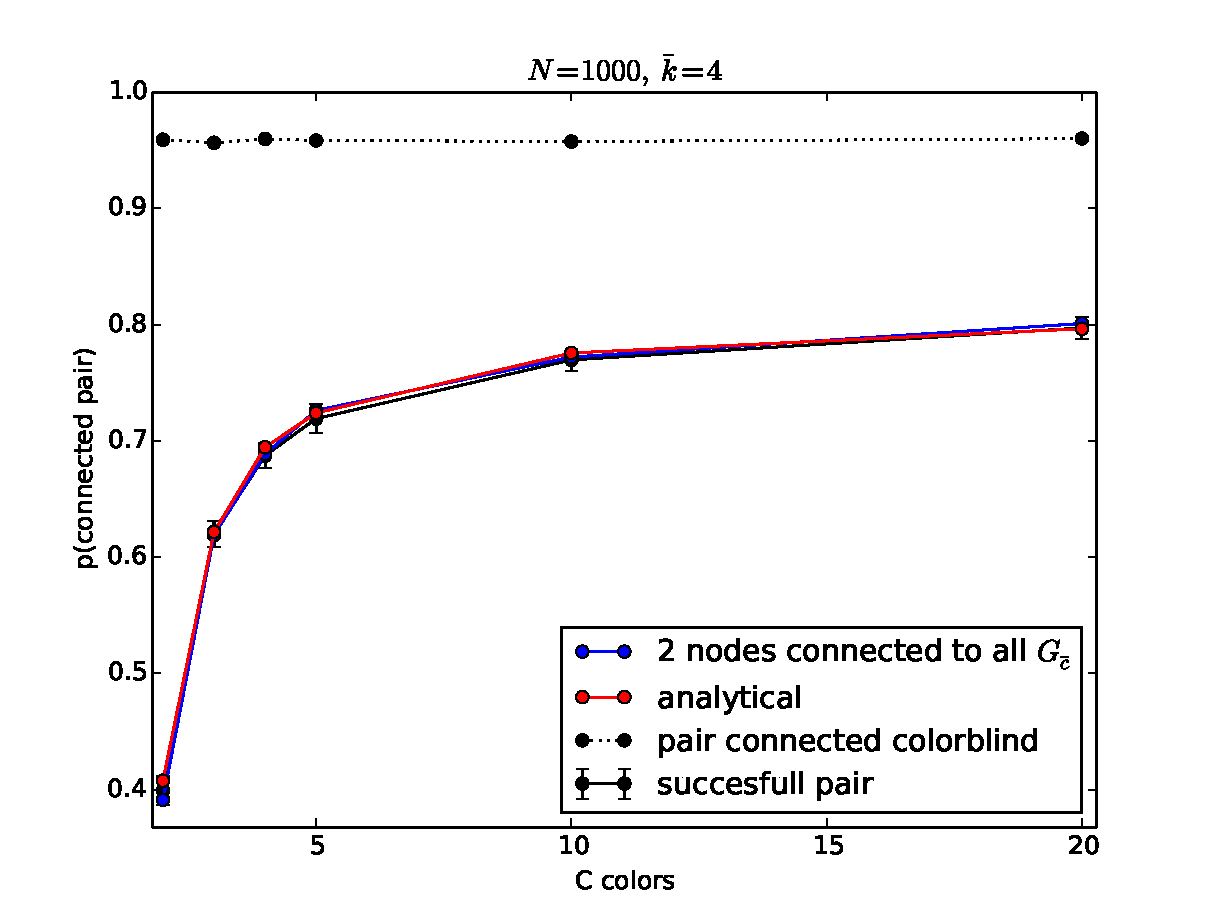
\includegraphics[width=0.7\columnwidth]{finder_C.pdf}
	\caption{Fraction of node pairs connected with color avoiding paths as described 
	in the text. Colors are distributed randomly on Poisson graphs with average degree 
	${\bar k}=4$. Black symbols with error bars show results for networks of size 
	$N=1000$, with samples of 200 node pairs, averaged over 50 networks. Connected pairs 
	are suppressed compared to the existence of colorblind paths, as indicated with 
	black symbols. 
	Blue symbols show the fraction of node pairs where each node is connected 
	to color avoiding giant components, confirming 
	the understanding using percolation theory. Red symbols show analytical results 
	of percolation theory.}
	\label{fig:model}
\end{center}
\end{figure}
%
For numerical results, we generated Poisson graphs with $N=1000$ (we used the 
Poisson distribution as an approximation to the binomial distribution in 
ER-graphs), and distributed $C$ colors over the nodes, with $r_c=1/C$. 
To check for a single pair, if it can be connected in 
the way as described above, we removed all nodes with the first color (except for 
the node pair under consideration) and 
searched for the shortest path (using a library function returning an empty set, 
if no path exists). Then we took the original graph and removed all nodes with the 
second color etc. If for all colors the shortest path exists, we considered the 
pair as successful. The case of a successful pair with a smaller number of 
paths, where e.g. one path avoids two colors, is included, as such a path could 
just be counted twice with our procedure. We repeated this 200 times with node pairs 
randomly chosen, and calculated the fraction of successful node pairs. See the black 
straight line in figure~\ref{fig:model}, with averages over 50 network realizations. The dotted 
line shows the fraction of node pairs, which are connected with a path which can 
have all colors. 


\section{Theory}

\subsection{Connection to percolation}

For estimating the fraction of successful pairs analytically, results from percolation 
theory can be used. First of all, the existence of a (colorblind) giant component clearly is a 
prerequisite for the existence of a macroscopic fraction of successful node pairs. With the 
generating functions of degree $g_0(z)=\sum_k p_k z^k$ and excess degree 
$g_1(z)=\sum_k q_k z^k$, the size of the giant component $S$ can be calculated (assuming infinite
networks which are locally treelike) using 
the average probability $u$, ``that a vertex is not connected to the giant component 
via its connection to some particular neighboring vertex'' (Newman, page 461): 
\begin{align}
u &= g_1(u)\\
S &= 1 - g_0(u).\label{eq:gc}
\end{align}
Lets call the set of all nodes belonging to the giant component as ${\mathcal G}$. 
Another prerequisite is the existence of a giant component after deleting all nodes of one 
of the colors $c$. Lets call the analogue of $u$ after all nodes of color $c$ are 
deleted as $u_{\bar c}$, the set of all nodes in the remaining giant component as 
${\mathcal G}_{\bar c}$, and its size as $S_{\bar c}$. 
We have 
\begin{align}
\phi_{\bar c} &= 1-r_c\\
u_{\bar c} &= 1-\phi_{\bar c} + \phi_{\bar c} g_1(u_{\bar c})\label{eq:u_c}\\
S_{\bar c} &= \phi_{\bar c} (1-g_0(u_{\bar c})).
\end{align}
Finally a node pair is for sure successful, if for both nodes the following 
holds: For every color $c$ there exists at least one neighbor belonging to 
${\mathcal G}_{\bar c}$. Lets call the set of all nodes fulfilling this 
condition as ${\mathcal G}_{\rm color}$, and its size as $S_{\rm color}$. 
The fraction of successful node pairs should be approximately $S_{\rm color}^2$. 

We tested this hypothesis with numerical results. For every color $c$, we labeled all the 
nodes with a boolean variable, if they belong to ${\mathcal G}_{\bar c}$ (more precise, if they 
belong to the largest component, as the networks are finite). A single node can 
belong to different components ${\mathcal G}_{\bar c}$. Then we searched for 
nodes which can be successful in a node pair. For a single node, we iterated over 
all the neighbors and collected all the memberships ${\mathcal G}_{\bar c}$ present. If for 
all colors $c$ there is at least one membership ${\mathcal G}_{\bar c}$ among the neighbors, 
the node belongs to ${\mathcal G}_{\rm color}$ and is
potentially successful in a pair. We calculated the 
fraction $S_{\rm color}$ over all nodes, and by squaring this we got an estimate for 
successful node pairs. This procedure ignores paths in small components, but 
is a good estimate, as can be seen with the blue line in figure~\ref{fig:model}. 
This procedure is much faster as well.


\subsection{Analytical results for the percolation problem}

As we have tested numerically that $S_{\rm color}$ can be used to describe the success of node 
pairs in connecting over paths with avoided colors, it is useful to assess this quantity 
analytically. We will do this assuming an infinite, locally treelike network. 
We calculate $S_{\rm color}$ as the probability, that a randomly chosen node belongs to 
${\mathcal G}_{\rm color}$. 

Let us start with the standard percolation theory. We can rewrite eq.~\ref{eq:gc} for the size of 
the giant component as 
%%%
\begin{align}
S &= \sum_{k=0}^{\infty}p_k \sum_{k'=0}^{k} B_{k,k'} \times \left( 1-\delta_{k',0}\right),\\
B_{k,k'} &={k \choose k'}(1-u)^{k'}u^{k-k'},
\end{align}
%%%
where $p_k$ is the probability that a randomly chosen node has exactly $k$ links and $B_{k,k'}$
is the binomial probability that out of these links $k'$ links connect to the giant component. The 
success probability $\left( 1-\delta_{k',0}\right)$ is zero 
if there is no link connecting to the giant component and one else. 
For our problem, this last term has to be replaced. In order to calculate 
the probability that the $k'$ links connect to all components ${\mathcal G}_{\bar c}$, 
we first have to consider the distribution of colors among the nodes these links connect to. 
%%%
\begin{align}
M_{k',\vec \kappa} &=\frac{k'!}{\kappa_1! \times \dots \times \kappa_C!} \,
(r_1)^{\kappa_1} \times \dots \times (r_C)^{\kappa_C}\,
\delta_{k',\kappa_1+\dots + \kappa_C}\label{eq:R_kk}
\end{align}
%%%
denotes the multivariate probability that out of those $k'$ links $\kappa_1$ connect to nodes of 
color 1, $\kappa_2$ links connect to nodes of color 2 etc. We define $P_{\vec \kappa}$ as the 
success probability to connect to all components ${\mathcal G}_{\bar c}$ given $\vec \kappa$. 
With this quantity, which will be evaluated below, we finally can write 
%%%
\begin{align}
S_{\rm color} &= \sum_{k=0}^{\infty}p_k \sum_{k'=0}^{k} B_{k,k'} 
\sum_{\kappa_1,\dots, \kappa_C=0}^{k'} M_{k',\vec \kappa} 
P_{\vec \kappa}.\label{eq:s_color}
\end{align}

For evaluating $P_{\vec \kappa}$, lets first concentrate on one color $c$. We have 
$\sum_{c'\neq c}\kappa_{c'}$ links which potentially can connect to the desired component ${\mathcal G}_{\bar c}$. 
According to the choices we have made so far, those links connect to the giant component 
${\mathcal G}$ and none of the nodes they are connecting to has color $c$. Therefore, a single 
of those links fails in connecting to ${\mathcal G}_{\bar c}$ with the conditional probability 
%%%
\begin{align}
U_{\bar c} &= 1 - \frac{1-u_{\bar c}}{(1-u)(1-r_c)}.\label{eq:U_c}
\end{align}
%%%
The last term is the probability, that over a single link a connection to ${\mathcal G}_{\bar c}$
is established, if this link already fulfills the following precondition: 
It connects to ${\mathcal G}$ and at the same time to a node without color $c$. 
This precondition has probability $(1-u)(1-r_c)$, as colors are randomly distributed and therefore 
are not correlated with the probability $u$ or $1-u$. As the links connecting to ${\mathcal G}_{\bar c}$ 
are a subset of all links fulfilling the precondition, the conditional probability can be 
calculated by dividing with the probability of the precondition. 
Notice that the additional information of the explicit color, instead of only stating that the color 
is not $c$, does not alter the results, as a further restriction of the colors 
would meat the numerator and denominator identically and therefore would cancel out. 
There is at least one link connecting to ${\mathcal G}_{\bar c}$ with probability 
$1-(U_{\bar c})^{\sum_{c'\neq c} \kappa_{c'} }$. The success probabilities for different colors have to be 
multiplied, as all ${\mathcal G}_{\bar c}$ have to be reached at the same time. 
Putting everything together we have 
%
\begin{align}
P_{\vec \kappa} &= \prod_{c=1}^C [1-(U_{\bar c})^{\sum_{c'\neq c} \kappa_{c'} }].\label{eq:p_success}
\end{align}

Results for Poisson graphs are shown in figure~\ref{fig:model} with the red line, showing 
$S_{\rm color}^2$ as the probability of two nodes to be connected via all Components 
$G_{\bar c}$ simultaneously. Instead of evaluating the sums over $k'$ and $\vec \kappa$ 
in eq.~\ref{eq:s_color}, we sampled 5000 events for every $k$.The outcome compares well with 
numerical results. 

\subsection{Limiting case of small color frequencies}

In the limit of high numbers of colors $C$ together with color frequencies $r_c \to 0$, the 
single paths have to avoid only a small part of nodes. Therefore we expect $U_{\bar c}\to 0$: If a 
link connects to the colorblind giant component, it will almost never fail to connect to 
the color avoiding component. Accordingly $P_{\vec \kappa}$ is close to one, if the needed 
links exist. We can use this idea to find a limiting case for $S_{\rm color}$ in eq.~\ref{eq:s_color}, 
and to compare to standard percolation. With the upper limit 
%%%
\begin{align}
\sum_{\kappa_1,\dots, \kappa_C=0}^{k'} M_{k',\vec \kappa} 
P_{\vec \kappa} &\leq 1-\delta_{k',0}-\delta_{k',1}
\end{align}
%%%
and $\sum_{k}p_k \sum_{k'} B_{k,k'} \sum_{\kappa_1,\dots, \kappa_C} M_{k',\vec \kappa} = 1$ 
(total probability is one) we finally get 
%
\begin{align}
S_{\rm color} &\leq 1-\sum_{k=0}^{\infty}p_k [u^k +k (1-u) u^{k-1}]\\
 &= 1 - g_0(u) - (1-u) \left.\frac{{\rm d}g_0(z)}{{\rm d}z}\right|_{z=u}\\
 &= S_{{\rm color},\infty}.\label{eq:limit}
\end{align}
%
The upper limit $S_{{\rm color},\infty}$ for $S_{\rm color}$ reflects the fact, that every node has to be 
connected to the giant component at least over two links. It therefore includes a reduction 
compared to the standard percolation result $1-g_0(u)$. In the limit of many colors and small 
probabilities $r_c$, $S_{\rm color}$ can come close to $S_{{\rm color},\infty}$, as in this case $U_{\bar c}$ comes 
close to zero and only nodes fail which have less than two links connecting to the giant component. 
This result is closely connected to $k$-core percolation with $k=2$. Note that $k$-core percolation shows 
a continuous phase transition for $k=2$, and only for $k>2$ has the well known discontinuous behavior. 

\subsection{Degree-dependent color distributions}\label{subsec:degree}

Our framework can be generalized to color distributions  
${\tilde r}_{c,k}$ additionally depending on the degree $k$ of the nodes. For an easier overview 
here all the needed equations. The following equations stay unchanged, 
%%%
\begin{align}
S_{\rm color} &= \sum_{k=0}^{\infty}p_k \sum_{k'=0}^{k} B_{k,k'} 
\sum_{\kappa_1,\dots, \kappa_C=0}^{k'} M_{k',\vec \kappa} 
P_{\vec \kappa},\\
B_{k,k'} &={k \choose k'}(1-u)^{k'}u^{k-k'},\\
u &= g_1(u),\quad g_1(z)=\sum_k q_k z^k,\\
M_{k',\vec \kappa} &=\frac{k'!}{\kappa_1! \times \dots \times \kappa_C!} \,
(r_1)^{\kappa_1} \times \dots \times (r_C)^{\kappa_C}\,
\delta_{k',\kappa_1+\dots + \kappa_C},\\
P_{\vec \kappa} &= \prod_{c=1}^C [1-(U_{\bar c})^{\sum_{c'\neq c} \kappa_{c'} }],\\
U_{\bar c} &= 1 - \frac{1-u_{\bar c}}{(1-u)(1-r_c)},
\end{align}
%%%
while including modified quantities $r_c$ and $u_{\bar c}$ according to 
%%%
\begin{align}
r_c &= \sum_k k p_k {\tilde r}_{c,k}/{\bar k},\\
u_{\bar c} &= 1- f_1(1) +  f_1(u_{\bar c}),\quad f_1(z)=\sum_k q_k (1-{\tilde r}_{c,k+1}) z^k.
\end{align}
%%%
$r_c$ is the average probability to find color $c$ over a link, including the fact that 
high degree nodes are reached more probably and therefore the colors on high degree nodes 
are found with higher probability. The self-consistency equation for $u_{\bar c}$ is 
well known from standard percolation theory. 



\section{Results}

\subsection{Poisson graphs}


\begin{figure}[htb]
\begin{center}
	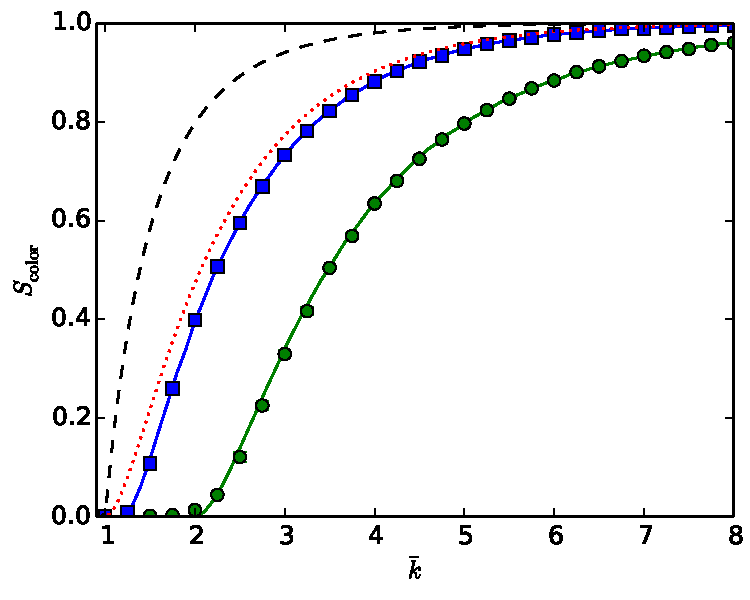
\includegraphics[width=0.5\columnwidth]{S_color_poisson.pdf}
	\caption{Dependence of $S_{\rm color}$ on the average degree for different number of colors. 
	Symbols show numerical results for networks of size $N=1000$ 
	(blue squares for $C=10$ and green circles for $C=2$ colors), 
	the straight lines show the according analytical results. For comparison, 
	the giant component size $S$ is shown (black dashed). $S_{\rm color}$ is reduced due to two mechanisms: First, 
	every node has to be connected to the giant component via two links. The according fraction of 
	nodes $S_{{\rm color},\infty}$ is shown with a red dotted line. Second, increasing color frequencies 
	further decrease $S_{\rm color}$.}
	\label{fig:poisson}
\end{center}
\end{figure}

In figure~\ref{fig:poisson} the dependence of $S_{\rm color}$ on the average degree is shown for different numbers 
of colors $C$ ($r_c=1/C$). Comparing to the standard giant component size $S$ (dashed black line in the figure), 
the percolation sets in at increasing $\bar k$ with smaller numbers of colors, and the component size grows 
slower to the saturation value of one. The symbols show numerical results with $N=1000$ and 100 network realizations, 
the lines show results of equation~\ref{eq:s_color}, both correspond well. 

The suppression of the number of connected nodes can be understood as a combination of two effects. 
The first effect is purely topological and can be understood with $S_{{\rm color},\infty}$ of eq.~\ref{eq:limit}
(shown with dotted red line). It means that only nodes can belong to $S_{\rm color}$, which are connected 
to the colorblind giant component over at least two links. We can confirm that 
$S_{\rm color}$ comes close to $S_{{\rm color},\infty}$ for high numbers of colors $C$ with the results for $C=10$.
$S_{{\rm color},\infty}$ is remarkably reduced compared to $S$ for small $k$, but has the same critical parameter. 
For the Poisson graph we have $g_0(z)=\exp({\bar k}(z-1))$ and $S=1-u$ and therefore 
$S_{\rm color,\infty}=S-{\bar k} S (1-S)$, and for small positive ${\bar k}-1$ 
the giant component grows approximately with $S\approx 2 ({\bar k}-1)/{\bar k}^2$. Therefore
\begin{align}
S_{\rm color,\infty}\approx 2({\bar k}-1)^2/\bar k,
\end{align}
which grows slowly for small parameter ${\bar k}-1$. 

The second effect is connected to finite color frequencies $r_c$ which further reduces the percolating 
fraction of nodes. This also changes the critical value ${\bar k}_{\rm crit}$ and the critical exponent 
$\beta$. We will discuss the critical behavior for the more general case of heterogeneous color 
distributions $r_c$. 




\begin{figure}[htb]
\begin{center}
    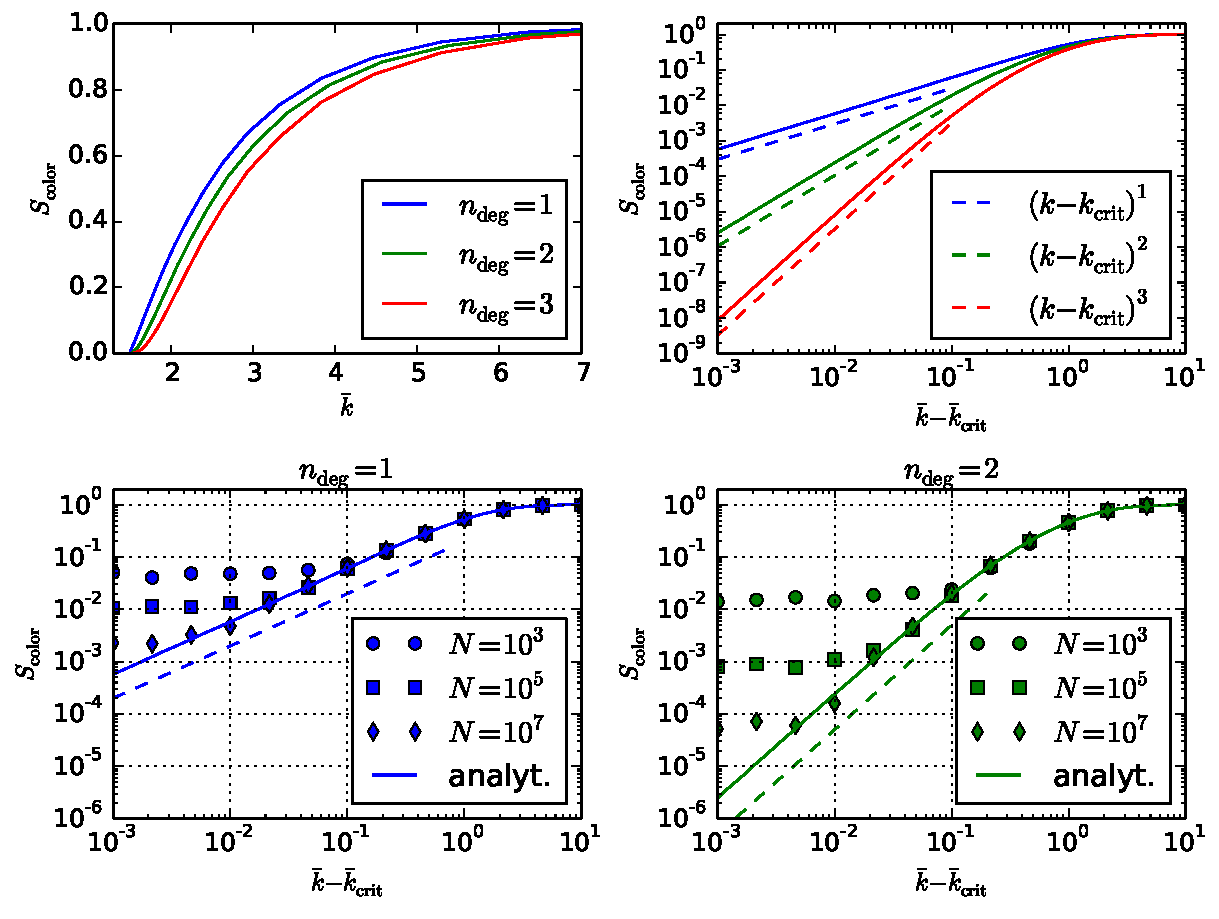
\includegraphics[width=0.7\columnwidth]{S_color_heterogen.pdf}
    \caption{For heterogeneous color distributions $r_c$, the highest frequency determines the behavior. 
    On the upper left, analytical results for Poisson graphs are shown for different color distributions 
    with $\max_c r_c=1/3$ and $C=10$, all with the same 
    ${\bar k}_{\rm crit}=1/(1-\max_c r_c)=3/2$. The critical exponent is determined by the degeneration 
    of the highest color frequency. On the upper right, the same results are shown with a log-log plot
    confirming $\beta=n_{\rm deg}$. This can be understood with an expansion of equation~\ref{eq:s_color}. 
    On the bottom, the analytical results are compared to numerical results which converge to the 
    expected critical behavior with system size.}
    \label{fig:pt}
\end{center}
\end{figure}



With general color distributions $r_c$ ($\sum_c r_c =1$), the color with the largest probability 
$r_c$ dominates 
the behavior, as it corresponds to the largest conditional link failure probability $U_{\bar c}$
in equation~\ref{eq:p_success}. For Poisson graphs, $U_{\bar c}$ 
falls below one at ${\bar k}=1/(1-r_c)$, and as long as one $U_{\bar c}$ is one, equation~\ref{eq:p_success}
gives always zero. Therefor the critical value is 
\begin{align}
{\bar k}_{\rm crit}=1/(1-\max_c r_c).
\end{align}
In figure~\ref{fig:pt} upper left, analytical results for a highest color frequency $r_1=1/3$ are shown. 
The corresponding critical value is ${\bar k}_{\rm crit}=1/(1-\max_c r_c)=3/2$ as expected. 
Different color distributions were used with different degeneration $n_{\rm deg}$ of the highest color 
frequency and $C=10$ colors. We see the same critical value, but different critical exponents $\beta = n_{\rm deg}$ for 
$S_{\rm color} \propto ({\bar k}-{\bar k}_{\rm crit})^{\beta}$.
This analytical result can be confirmed with numerical results, as shown on the bottom of the figure. 


We can understand the critical exponent with expanding equation~\ref{eq:p_success} using 
$U_{\bar c}=1-\varepsilon$ for the highest color frequency. 
We will show below using results from standard percolation that 
$\varepsilon\propto ({\bar k}-{\bar k}_{\rm crit})$. First of all, we have 
$(U_{\bar c})^{\sum_{c'\neq c} \kappa_{c'} }\approx 1-({\sum_{c'\neq c} \kappa_{c'} })\times \varepsilon$, and therefore we find 
$P_{\vec \kappa} \propto \varepsilon^{n_{\rm deg}}$ (unless $P_{\vec \kappa} = 0$ in the case ${\sum_{c'\neq c} \kappa_{c'} }=0$
for any $c$). As equation~\ref{eq:s_color} is therefore a superposition of either vanishing terms or terms with 
leading order $\varepsilon^{n_{\rm deg}}$, we have 
%%%
\begin{align}
\beta=n_{\rm deg}.
\end{align}
%%%
To complete the discussion of the critical behavior, we have to show that 
$1- U_{\bar c}\propto ({\bar k}-{\bar k}_{\rm crit})$ for a certain region of critical behavior. 
We know from standard percolation theory for Poisson graphs that $S \propto ({\bar k}-1)^1$, and therefore 
$1-u({\bar k})\approx a \times ({\bar k}-1)$ for $\bar k$ exceeding the critical value 
about small values. With inserting into equation~\ref{eq:u_c} it can be shown that 
$u_{\bar c}({\bar k})=1-\phi_{\bar c}+\phi_{\bar c}u({\bar k}\phi)$. Using this in 
equation~\ref{eq:U_c} ($\phi_{\bar c}=1-r_c$), we find 
%%%
\begin{align}
U_{\bar c} &= 1 - \frac{1-u({\bar k}\phi_{\bar c})}{1-u({\bar k})}\\
&\approx 1- \phi_{\bar c} \frac{{\bar k}-{\bar k}_{\rm crit}}{{\bar k}-1}
\end{align}
%%%
which drops linearly from one in the critical region
%%%
\begin{align}
0< {\bar k}-{\bar k}_{\rm crit} &\ll {\bar k}_{\rm crit}-1.
\end{align}
%%%
In figure~\ref{fig:pt} we have ${\bar k}_{\rm crit}-1=1/2$, and critical behavior up to 
about ${\bar k}-{\bar k}_{\rm crit}=1/10$.

As a final remark let us discuss the critical behavior for largest color frequencies which 
are not perfectly degenerated. Lets assume two colors with close by values 
${\bar k}_1< {\bar k}_2$, where $U_{\bar c}$ drops below one. With equation~\ref{eq:p_success} and the definition 
$\varepsilon={\bar k}-{\bar k}_2$ we have above ${\bar k}_2$ that 
$P_{\vec \kappa} \propto \varepsilon \times (\varepsilon+({\bar k}_2 - {\bar k}_1))$. This 
is dominated by a linear term for small $\varepsilon$ and by a quadratic term for larger 
values, the crossover is at about
%%%
\begin{align}
{\bar k}-{\bar k}_2 &= {\bar k}_2-{\bar k}_1.
\end{align}
%%%
Exceeding the critical value ${\bar k}_{\rm crit}={\bar k}_2$ about more than the 
distance ${\bar k}_2 - {\bar k}_1$, $S_{\rm color}$ behaves as 
if the color frequencies would be degenerated. 

With these results altogether we can understand the behavior of $S_{\rm color}$ 
for small frequencies of all colors (compare to the blue squares and line in 
figure~\ref{fig:poisson} with $r_c=1/10$ for all colors). There is a deviation 
from $S_{{\rm color},\infty}$ due to $S_{\rm color}=0$ below ${\bar k}_{\rm crit}$, and 
above there is a region of slow critical growth with large critical exponent $\beta$. This region acts as an effective 
shift of the critical parameter. Further increasing $\bar k$, $U_{\bar c}$ saturates smoothly to zero for all colors. 
Accordingly, $S_{\rm color}$ has a smooth rise to finite values, but not governed by a certain critical exponent. 
It comes closer to $S_{{\rm color},\infty}$ without reaching it, as there are other effects (e.g. nodes with 
exactly two links can connect to two nodes of the same color). The smaller the highest color frequencies are, 
the closer $S_{\rm color}$ is to $S_{{\rm color},\infty}$.



%\clearpage


\subsection{Broad degree distribution}

\begin{figure}[htb]
\begin{center}
    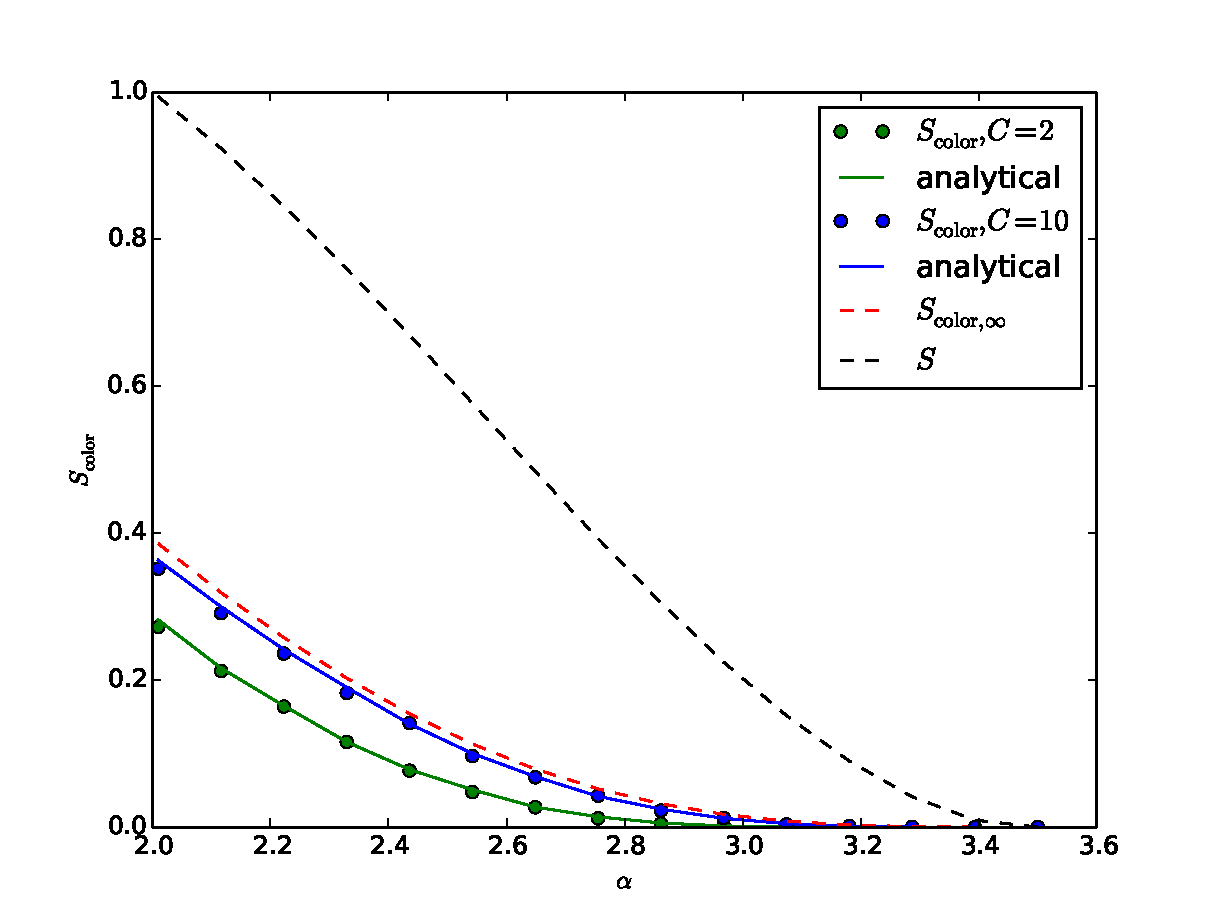
\includegraphics[width=0.6\columnwidth]{S_color_broad.pdf}
    \caption{The same as in figure~\ref{fig:poisson} for scale free degree distributions. }
    \label{fig:broad}
\end{center}
\end{figure}

In figure~\ref{fig:broad}, results for graphs with broad degree distributions with 
$p_k=n k^{-\alpha}$ are shown. $n$ is a normalization constant. We see a strong reduction of 
$S_{{\rm color},\infty}$ compared to $S$, while the number of colors ($r_c=1/C$) plays 
a minor role. Numerical results are averages over 50 networks of size $N=10\,000$. 
For evaluating equation~\ref{eq:s_color}, 1000 events where sampled for every $k$. 


\begin{figure}[htb]
\begin{center}
	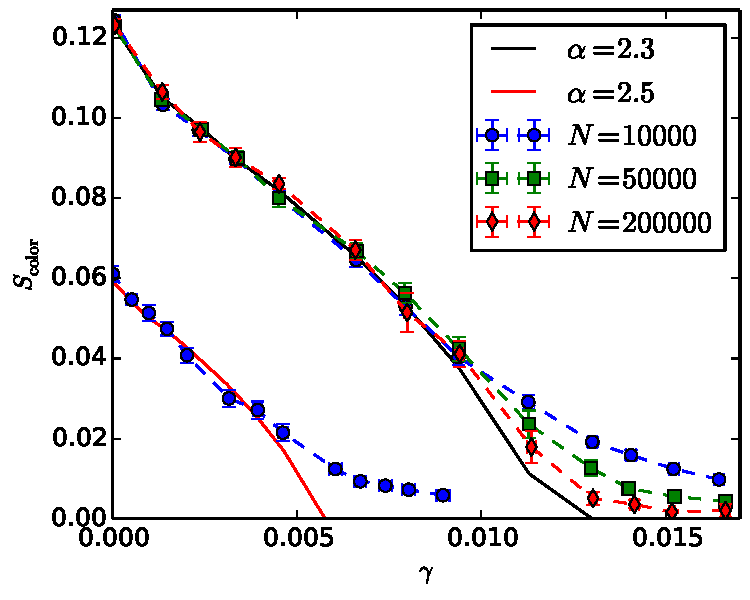
\includegraphics[width=0.49\columnwidth]{S_color_degree_dependent_broad.pdf}
    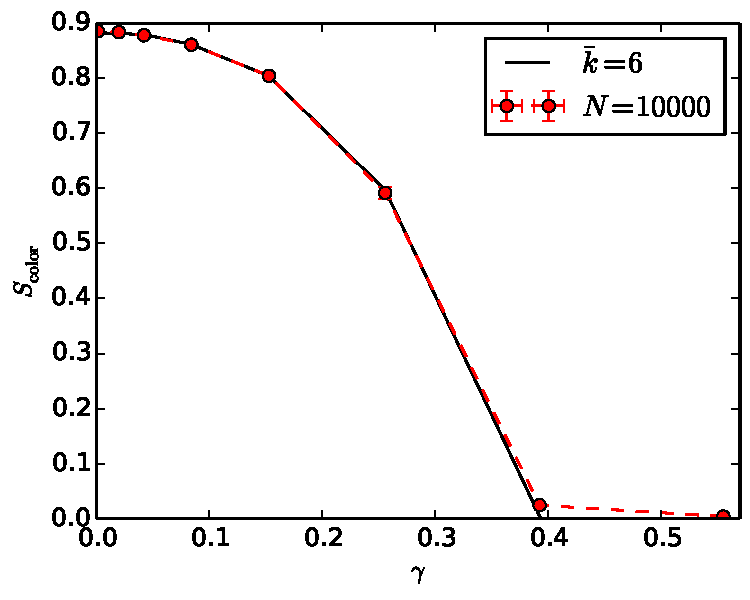
\includegraphics[width=0.49\columnwidth]{S_color_degree_dependent_poisson.pdf}
	\caption{Left: On graphs with broad degree distribution, $S_{\rm color}$ drops fast, 
	if a fraction $\gamma$ of nodes with the highest 
	degree is restricted to one color, while the nodes with smaller degree can have one of 
	two colors. This is shown for networks with $\alpha=2.3$ and $\alpha=2.5$ having $N=10000$ 
	with symbols. Analytical results need the modified version of equation~\ref{eq:s_color} 
	as described in section~\ref{subsec:degree}. Results are shown with straight lines. Without diversity 
	on the hubs, nodes cannot communicate in the desired way. Right: For comparison results on a Poisson 
	graph are shown, where a large fraction of nodes has to be of one color to hinder communication.}
	\label{fig:degree}
\end{center}
\end{figure}

For broad degree distributions, color distributions can show an additional type of 
heterogeneity, as a dependence of frequencies on the degree of a node can strongly 
influence the behavior. We used two colors, where the first color has a frequency 
of ${\tilde r}_{1,k}=1$ for all degrees $k\geq k_{\rm step}$ larger than a certain 
$k_{\rm step}$. These nodes have a probability of 
$\gamma=\sum_{k=k_{\rm step}}^{\infty} p_k$. Accordingly 
${\tilde r}_{2,k}=0$ for $k\geq k_{\rm step}$, and probabilities for smaller degrees are chosen as 
${\tilde r}_{c,k}=1/2$. Figure~\ref{fig:degree} on the left shows results for an ensemble with 
$\alpha=2.3$ and $\alpha=2.5$. The analytical results for $\alpha=2.3$ show that already for a portion 
of $\gamma=1.4\%$ of the largest nodes occupied by the first color exclusively, $S_{\rm color}$ vanishes. 
These results were calculated as described in section~\ref{subsec:degree}. 
Numerical results confirm this behavior, but show finite size effects. 
On the right of the figure, results for Poisson graphs are shown. We see that for narrow 
degree distributions the effect of dominance of one color on the nodes of highest degrees 
is much smaller. Therefore, graphs with narrow degree distributions are much more robust 
for providing connection over color avoiding paths. 



\subsection{Application: Network of autonomous systems}

\begin{figure}[htb]
\begin{center}
    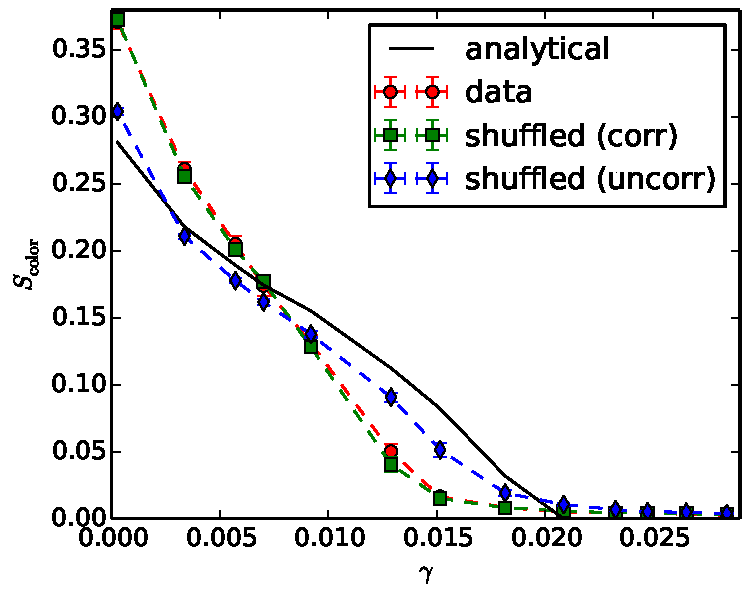
\includegraphics[width=0.49\columnwidth]{S_color_degree_dependent_data.pdf}
    \caption{Red circles show results for the network of autonomous systems, where colors are 
    distributed in the same way as in figure~\ref{fig:degree}. Averages were taken over 10 color 
    distributions. Analytical results are shown with the black line and reproduce the results qualitatively. 
    Deviations are due to degree-degree-correlations which are reserved in shuffled networks shown 
    with green squares, while results with ignoring correlations are shown with blue diamonds.}
    \label{fig:as}
\end{center}
\end{figure}

The red circles in figure~\ref{fig:as} show results for the autonomous systems network, where colors 
where distributed with degree-dependence over the nodes as described at the end of the last section. 
Averages where taken over 10 realizations of the color distributions. As expected from our results 
for scale free degree distributions, $S_{\rm color}$ drops to 0 even for small fraction $\gamma$ 
which is exclusively of one color. That means that if there is no heterogeneity in the highly 
connected servers, it is not possible to avoid e.g. software versions. This is also 
interesting in the following sense: It is known that secret services try to store all decrypted data 
running through servers to decrypt it later. As this is connected to technical afford, 
the services will more likely monitor the large servers. Therefore it would be beneficial, if once 
using encryption, to sent parts of the message using small servers. Unfortunately, this seems to 
be impossible, the services only have to monitor a low percentage of servers to hinder alternative 
paths. 

In order to assess the predictive power of our analytical method, we used a model ensemble with 
using the degree frequencies of the autonomous systems network as degree distribution $p_k$. 
Results for the according ensemble are shown with the black line. The qualitative 
behavior is represented well. To understand deviations, we compared to data from shuffled networks 
starting with the original data. Shuffling with ignoring degree-degree-correlations while only 
keeping the degree sequence gives results close to the analytical results (blue diamonds). 
Shuffling with also keeping degree-degree-correlations gives results close to the original network 
(green squares). 
Therefore, deviations between our theory and the data arise mainly due to degree-degree-correlations. 



\section*{Appendix: Independence of components for Poisson graphs}

In equation~\ref{eq:s_color}, the probabilities $1-U_{\bar c}^{k'-k_c}$ for 
different colors may show dependencies 
among each other limiting the usability of the equation. In the following we 
discuss one particular case for Poisson graphs, in order to illustrate a sort 
of independence. Lets assume we only have one link connecting to a node in the 
giant component, and the node has color 3. Can the probability, that this link connects 
to ${\mathcal G}_{\bar 1}$ and ${\mathcal G}_{\bar 2}$ at the same time 
really be written as the product $(1-U_{\bar 1})(1-U_{\bar 2})$? 
As for Poisson graphs we 
have $S=1-u$, instead of discussing link probabilities $u$ we can concentrate on 
node probabilities $S$. 

We use the notation $S\left({\mathcal Y}\middle|{\mathcal X}\right)$ to denote 
the fraction of nodes in a set ${\mathcal Y}$ which is a subset of ${\mathcal X}$. With 
the set ${\mathcal N}$ of all nodes in the network we have 
$S_{\bar c}=S\left({\mathcal G}_{\bar c}\middle|{\mathcal N}\right)$. Clearly they must 
be dependent, as 
$S\left({\mathcal G}_{\bar 1}\cap {\mathcal G}_{\bar 2}\cap \dots 
\cap {\mathcal G}_{\bar C}\middle| {\mathcal N}\right)=0\neq 
S\left({\mathcal G}_{\bar 1}\middle| {\mathcal N}\right)\times\dots \times 
S\left({\mathcal G}_{\bar C}\middle| {\mathcal N}\right)$. 
Lets call the set of all nodes with color c as ${\mathcal A}_c$, 
and the set of all nodes without this color as ${\mathcal A}_{\bar c}$. 

Back to our case with the Poisson graph, we have for $c=1,2$
\begin{align}
1-U_{\bar c} &=\frac{S_{\bar c}}{S (1-r_c)}\\
 &= S\left({\mathcal G}_{\bar c} \cap {\mathcal A}_{\bar c} \middle| {\mathcal G} \cap {\mathcal A}_{\bar c} \right)\\
 &= S\left({\mathcal G}_{\bar c} \cap {\mathcal A}_{3} \middle| {\mathcal G} \cap {\mathcal A}_{3} \right).
\end{align}
The last equation is intuitive, as the coloring of nodes is random, and it was tested numerically (results not shown). 
In order to test if the product $(1-U_{\bar 1})(1-U_{\bar 2})$ reflects the probability of 
connecting to ${\mathcal G}_{\bar 1}$ and ${\mathcal G}_{\bar 2}$ at the same time, 
we have to check if 
\begin{align}
S\left({\mathcal G}_{\bar 1}\cap {\mathcal G}_{\bar 2} \cap {\mathcal A}_3 \middle| {\mathcal G} \cap {\mathcal A}_3 \right)=
S\left({\mathcal G}_{\bar 1} \cap {\mathcal A}_3 \middle| {\mathcal G} \cap {\mathcal A}_3 \right)\times 
S\left({\mathcal G}_{\bar 2} \cap {\mathcal A}_3 \middle| {\mathcal G} \cap {\mathcal A}_3 \right)\label{eq:independent}
\end{align}
holds. The comparison of the left hand side and the right hand side 
is shown in figure~\ref{fig:corr} for networks with $N=1000$. For every number of colors $C=3,4,5,10$, 
ten network realizations were used. So we have tested numerically, that 
equation~\ref{eq:s_color} is useful at least in this very simple case. This was 
to illustrate a sort of independence of the conditional probabilities for connecting 
to color-avoiding giant components. The generalization to many links and 
general degree distributions is missing so far. 



\begin{figure}[htb]
\begin{center}
	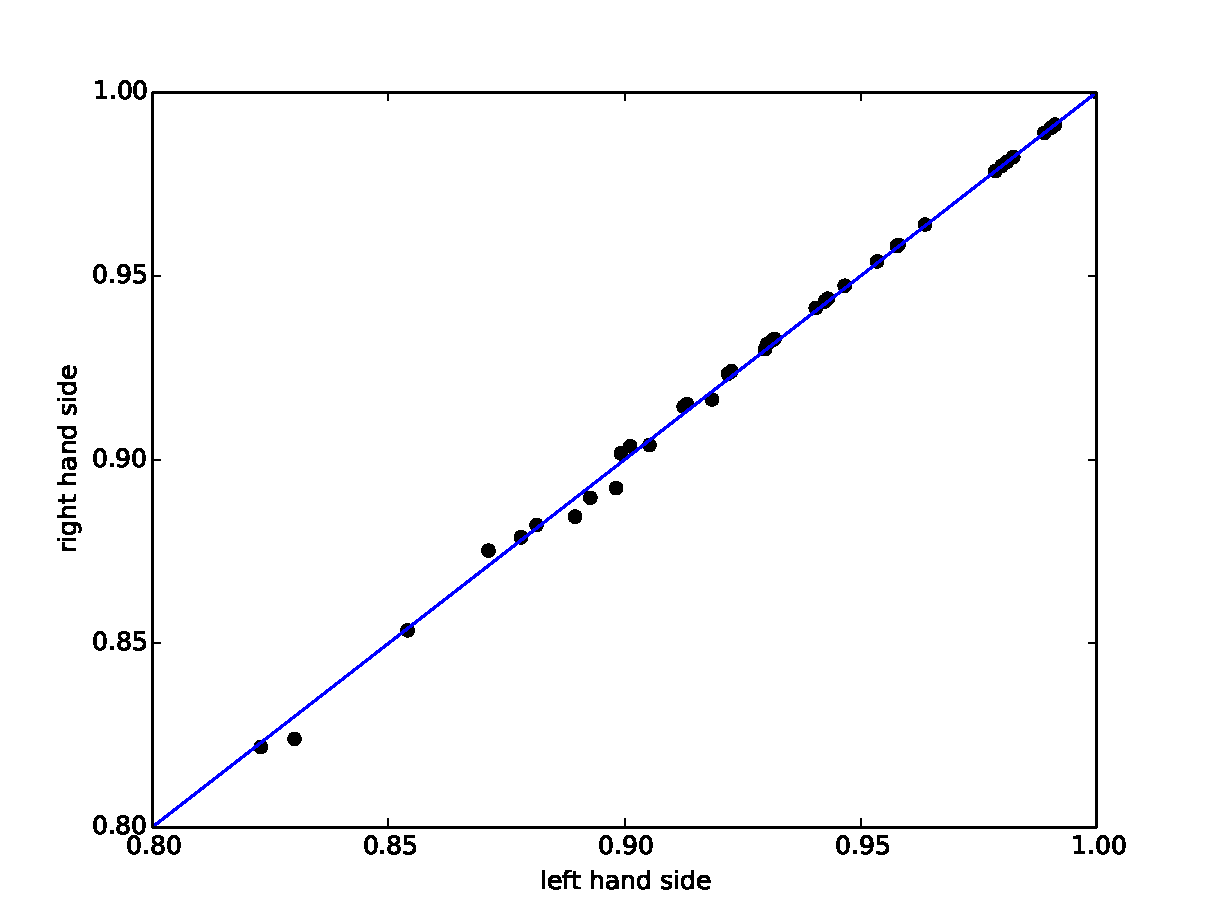
\includegraphics[width=0.6\columnwidth]{finder_C_correlated.pdf}
	\caption{Calculating both sides of equation~\ref{eq:independent} for Poisson networks with $N=1000$ 
	motivates the usage of the conditional probabilities $U_{\bar c}$ as independent quantities.}
	\label{fig:corr}
\end{center}
\end{figure}


\bibliographystyle{apsrev4-1}
\bibliography{mp}

\end{document}
